\chapter{Applications of Convolution to Different Data Types}

Convolutional networks are not limited to images.  
The same mathematical operation can be applied to different data types, depending on their structure and dimensionality. In this section we review the most common cases.  

\section{One and Two dimensional data}

The simplest applications of convolution are to one-dimensional and two-dimensional arrays.  
In the one-dimensional case, typical of time series or audio signals, convolutional filters slide along the temporal axis, detecting short-term dependencies, periodicities or characteristic frequency components.  
This makes 1D convolution suitable for speech recognition, time-series forecasting and other tasks where local temporal context is important.  

In the two-dimensional case, characteristic of image data, the input is arranged in a grid of pixels (with additional channels for color).  
Here, convolutional kernels learn to capture local spatial features such as edges, textures and corners.  
By stacking multiple layers, the network progressively builds more complex and abstract representations, forming the foundation of modern computer vision systems.  

\section{Higher-dimensional data: video and volumetric analysis}
\label{sec:3D-CNNs}%

Convolution naturally extends to three or more dimensions.  
A key application is in video understanding, where the input has two spatial dimensions and one temporal dimension.  
In this case, 3D convolutional kernels are used to jointly model motion and appearance, enabling the detection of spatio-temporal patterns such as moving objects, gestures, or human actions.  

\clearpage

Ji et al. \cite{ji2013} proposed one of the first effective 3D CNN architectures for human action recognition.  
Their model performs convolutions over both spatial and temporal dimensions by applying 3D kernels to small cubes of consecutive video frames.  
This design captures motion features that are not accessible to standard 2D CNNs operating on individual frames.

\begin{figure} [H]
    \centering
    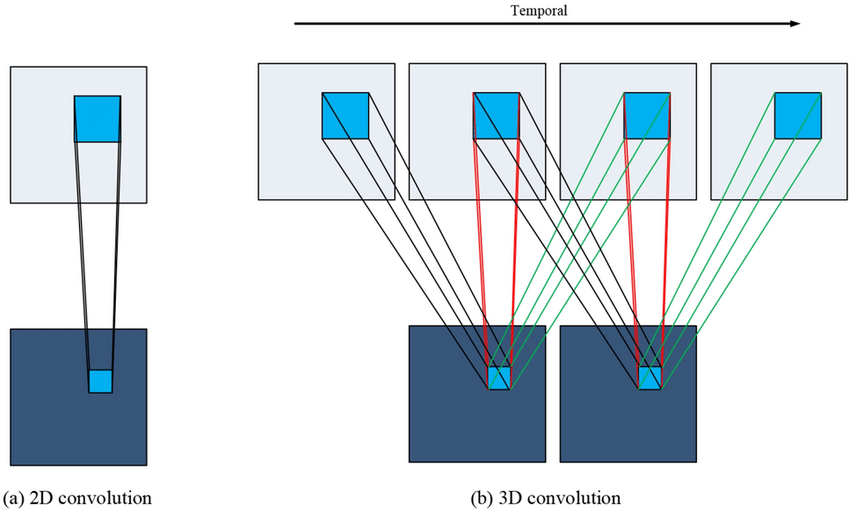
\includegraphics[width=0.7\linewidth]{Images//Chapters/Comparison-between-2D-CNN-and-3D-CNN.png}
    \caption{Comparison between 2D and 3D CNN}
    \label{fig:2Dvs3DCNN}
\end{figure}

Formally, the value at position $(x, y, z)$ on the $j$th feature map in the $i$th layer is given by

\begin{equation}
v^{xyz}_{ij} = \tanh \left( b_{ij} + 
\sum_{m} \sum_{p=0}^{P_i-1} \sum_{q=0}^{Q_i-1} \sum_{r=0}^{R_i-1} 
w^{pqr}_{ijm} \, v_{(i-1)m}^{(x+p)(y+q)(z+r)} \right),
\end{equation}

where $(P,Q,R)$ are the spatial and temporal dimensions of the kernel, $w^{pqr}_{ijm}$ are the kernel weights, and $b_{ij}$ is the bias.  

The proposed architecture was evaluated on large-scale datasets such as TRECVID surveillance videos and the KTH human action dataset. The results showed that 3D CNNs outperform traditional frame-based (2D CNNs) methods and handcrafted spatio-temporal features, particularly in real-world environments with cluttered backgrounds and viewpoint variations. Interestingly, the gains were more significant when the number of positive training examples was limited, highlighting the statistical efficiency of learned spatio-temporal features.

\clearpage